\documentclass[11pt,a4paper]{article}
\usepackage[margin=22mm]{geometry}
\usepackage{amsmath,amssymb,bm}
\usepackage{booktabs,longtable,array}
\usepackage{enumitem}\usepackage{graphicx}\usepackage{float}
\usepackage[hidelinks]{hyperref}
\usepackage{xcolor}
\usepackage[T1]{fontenc}
\usepackage[utf8]{inputenc}

% -----------------------------------------------------------------------------
% SST notation macros. Define notation here; only enter numerical constants when
% the blind protocol explicitly permits them.
% -----------------------------------------------------------------------------
\newcommand{\vswirl}{\mathbf{v}_{\!\boldsymbol{\circlearrowleft}}}
\newcommand{\rhoF}{\rho_{\!f}}
\newcommand{\rhoE}{\rho_{\!E}}
\newcommand{\rhoM}{\rho_{\!m}}
\newcommand{\rc}{r_c}

\title{UNASSIGNED --- Ruban $T(2,3)$ Reproduction\\Falsification Protocol and Final Report}
\author{SST-Workbench}
\date{30 October 2026 | v0.1.1}

\begin{document}
\maketitle

% SST-REPORT-SECTION:IDENTIFICATION

\section{Identification, scope, and status}
\begin{center}\begin{tabular}{ll}\toprule
Project & Ruban $T(2,3)$ publication reproduction\\
Version & v0.1.1\\
Catalog & UNASSIGNED (standalone, pending SST-Workbench admission)\\
Framework report template & v1.1.0 RC2, SST-FALSIFIER-RUNTIME-2\\
Framework execution & NOT EXECUTED; template-aligned development only\\
Scientific result & UNRESOLVED\\\bottomrule\end{tabular}\end{center}
\noindent\textbf{Report provenance.} This document is based on the authentic Framework v1.1.0 RC2 report template; it follows the section-marker/report-insertion contract, but the runtime snapshot, exact \texttt{FREEZE} validation and native certification were not installed or invoked. The scientific protocol is \textbf{not frozen}. No framework certification is claimed.

% SST-REPORT-SECTION:QUESTION

\section{Research question and objective}
Can the regularized Biot--Savart filament model of Ruban (2018), initialized as the analytical trefoil $T(2,3)$ at $B_0=0.154$, $\Lambda=1.4+\tfrac12\ln 200$ and $\delta/R_0=0.05$, achieve operational survival for dimensionless time $t\ge300$, translating more than $1200R_0$, without loss of numerical validity? This is a \emph{publication reproduction}, not a test of the full three-dimensional Euler equations, volume conservation of a thick tube or internal twist.

% SST-REPORT-SECTION:HYPOTHESES

\section{Competing hypotheses and allowed conclusions}
\textbf{$H_0$:} The published long-lived interval is not reproduced by the specified code and refinement schedule with the stated operational rules. \textbf{$H_1$:} A test at $B_0=0.154$ reaches $t\ge300$, $|z(t)-z(0)|\ge1200$ with acceptable conservation and resolved spatial/temporal error. If the solver violates numerical quality or the independent refinement is absent, the result is \textbf{UNRESOLVED}, not evidence against the physical claim. A partial run is not a test of survival beyond its attained time.

% SST-REPORT-SECTION:ASSUMPTIONS

\section{Assumptions, domain of validity, and known edge cases}
\begin{enumerate}[label=A\arabic*.]
\item Single closed analytical $T(2,3)$ filament in an unbounded fluid, with no externally imposed velocity.
\item Dimensionless units $R_0=1$ and circulation $\Gamma=2\pi$. Smooth closed periodic curve; one discretized centerline per seed.
\item Rosenhead-type regularization $\delta$ and a separate compensating local-induction coefficient; $\delta$ is not identified with the physical core radius.
\item Deterministic low-wavenumber perturbation with a recorded seed. Different resolutions and $B_0$ values are \emph{not} independent source providers.
\end{enumerate}
\noindent The limits $B_0\to0$ (non-embedded multiply traversed circle), $\delta\to0$ (regularization singularity), and underresolved near-contact geometries require separate analysis. No finite-core Euler or reconnection model is claimed.

% SST-REPORT-SECTION:SYMBOLS

\section{Symbols, units, and dimensional consistency}
\begin{center}\begin{tabular}{lll}\toprule Symbol & Meaning & Units here\\\midrule
$\mathbf X$ & filament centerline & $R_0$\\
$\beta$ & periodic parameter & dimensionless\\
$B_0$ & torus minor/major ratio & dimensionless\\
$\delta$ & Biot--Savart regularization & $R_0$\\
$\Lambda$ & physical slender-core logarithm & dimensionless\\
$\widetilde\Lambda_0$ & $\Lambda+\ln(\delta/R_0)$ & dimensionless\\
$t$ & normalized simulation time & $R_0^2/\Gamma$ scaling\\
$H$ & discretized filament Hamiltonian & normalized model energy\\\bottomrule\end{tabular}\end{center}
\noindent With physical circulation units $[\Gamma]=L^2T^{-1}$, the nonlocal line integral carries units $L^{-1}$ and is multiplied by $\Gamma$ to become velocity. In the chosen Ruban dimensionless convention, the integral coefficient is $1/2$; all computed coordinates and times are dimensionless. The local term has curvature units $L^{-1}$ and the same time-normalization scale.

% SST-REPORT-SECTION:EQUATIONS

\section{Exact mathematical model and observables}
\paragraph{E1 - continuous operator.}
\begin{equation}
\partial_t\mathbf X(\beta)=\frac12\int_0^{2\pi}\!\frac{\mathbf X_{\beta}(\beta')\times[\mathbf X(\beta)-\mathbf X(\beta')]}{(|\mathbf X(\beta)-\mathbf X(\beta')|^2+\delta^2)^{3/2}}\,d\beta'
+\frac{\widetilde\Lambda_0}{2}\frac{\mathbf X_\beta\times\mathbf X_{\beta\beta}}{|\mathbf X_\beta|^3} .\label{eq:E1}
\end{equation}
\paragraph{E2 - discrete update.} Fourier spectral derivatives in $\beta$, periodic trapezoidal quadrature over all samples (including the finite-regularization diagonal), and classical explicit fourth-order Runge--Kutta. The step is capped by an initial-value-model local-induction spectral bound evaluated on every accepted state:
\begin{equation}
\Delta t_{\rm allowed}=\min\left(\Delta t_{\rm requested},\;s\,\frac{4\sqrt{2}}{|\widetilde\Lambda_0|}\left(\frac{\min_i|\mathbf X_{i+1}-\mathbf X_i|}{\pi}\right)^2\right),\qquad s=0.4.\label{eq:E2}
\end{equation}
This is a \emph{heuristic conservative stability cap}, not a rigorous stability bound for the nonlocal coupled operator. The code also clips to upcoming diagnostic/output times; underflow and geometric degeneration stop the run.
\paragraph{E3 - discrete Hamiltonian and diagnostics.} The code uses the discretized Hamiltonian corresponding to the regularized interaction and local-induction term:
\begin{equation}
H = \frac{\pi}{2}\!\int_0^{2\pi}\!\int_0^{2\pi}\!
\frac{\mathbf X_\beta(\beta)\cdot\mathbf X_\beta(\beta')}
{\sqrt{|\mathbf X(\beta)-\mathbf X(\beta')|^2+\delta^2}}\,d\beta'\,d\beta
+\pi\widetilde\Lambda_0\int_0^{2\pi}|\mathbf X_\beta|\,d\beta.
\end{equation}
The double and single integrals are evaluated with periodic trapezoidal quadrature, using the same spectral derivatives as in E1.
\begin{equation}
\epsilon_H(t)=\frac{|H(t)-H(0)|}{\max(|H(0)|,10^{-12})},\quad
D(t)=\operatorname{RMS}_{\mathrm{rigid,cyclic}}(\mathbf X(t),\mathbf X(0)).\label{eq:E3}
\end{equation}
\paragraph{E4 - decision thresholds.} Require $\epsilon_H\le10^{-3}$, segment ratio $\max(\Delta s)/\min(\Delta s)\le10$, operational shape RMS $D\le0.25R_0$, $t\ge300$, $|\Delta z|\ge1200R_0$; thresholds are \emph{local operational choices}, not Ruban's unpublished termination rule. Diagnostics run at intervals no longer than $\Delta t_{\rm diag}=0.025$. Scientific qualification still requires convergence.
\IfFileExists{AUTO_SCIENCE_CONTRACT.tex}{\subsection*{Machine-readable equation register}
\begin{itemize}
\item \textbf{E1}: \texttt{ruban\_falsifier/model.py:RubanModel.velocity}, gate G2.
\item \textbf{E2}: \texttt{ruban\_falsifier/model.py,runner.py}, gate G2.
\item \textbf{E3}: \texttt{ruban\_falsifier/runner.py}, gate G2.
\item \textbf{E4}: \texttt{ruban\_falsifier/runner.py}, gate G3.
\end{itemize}\noindent Framework-runtime validation: NOT EXECUTED.
}{\emph{Machine-readable equation register is present in \texttt{configs/science\_contract.json}.}}

% SST-REPORT-SECTION:ALGORITHM

\section{Exact algorithm: equation-to-code mapping}
\begin{enumerate}[label=S\arabic*.]
\item Verify bundled input hashes and analytic seed parameters ($T(2,3)$, $B_0$).
\item Compute a ring symmetry benchmark with the same regularized filament operator.
\item Generate a torustrefoil at $N$ points, optionally with seeded smooth perturbation.
\item Evaluate all terms in Eq.~\eqref{eq:E1}, impose the step ceiling Eq.~\eqref{eq:E2} and integrate by Runge--Kutta.
\item Check geometry at every accepted step; energy and deformations at every diagnostic checkpoint.
\item Stop on the first failing numerical threshold, save a complete trace and closed-curve snapshots.
\item Evaluate independent spatial, temporal and regularization scans at fixed physical end time in a distinct campaign.
\item Record all gate results without promoting a short trial to the published long-time claim.
\end{enumerate}
\noindent Python/Numba float64 is a development reference only. No native C++ certification is present. Artificial damping, smoothing and remeshing are absent.

% SST-REPORT-SECTION:SOURCES

\section{Source, provenance, and independence contract}
Ruban (2018), \emph{Long-Lived Quantum Vortex Knots}, supplies the equations and target conditions. The local analytic $T(2,3)$ seed is one generated source family, not an independent provider. The user-supplied \texttt{3\_1.xyz} is hashed and retained for comparison but is not input to the time integrator. E010 v0.4.0 is geometry-only context. Numerical refinements of the same analytic seed are not independent replications. Exact input/source SHA-256 values accompany each run.

% SST-REPORT-SECTION:GATES

\section{Gate DAG and decision semantics}
\begin{center}\begin{tabular}{lp{0.70\linewidth}}\toprule Gate & Meaning\\\midrule
G0 & Provenance and input manifest\\
G1 & Circular-ring field symmetry\\
G2 & Numerical validity, energy, segment and step controls\\
G3 & Time $>300$ and travel $>1200R_0$ only with prerequisite numerical quality\\
G4 & Local $B_0$ stability window: withheld until proper lifetime comparison\\
G5 & Independent temporal/spatial convergence at equal final time\\
G6 & Publication-level numerical reproduction independent audit\\
G7 & Full finite-core Euler and internal core twist: not tested\\\bottomrule\end{tabular}\end{center}
\noindent Status categories: PASS, FAIL, UNRESOLVED, NOT\_TESTED. The local runtime does not claim the official v1.1.0 gate DAG, HMAC blindness, reveal phase or certification. For a numerically rejected run, the command exits nonzero even when source and ring gates PASS.

% SST-REPORT-SECTION:NUMERICS

\section{Numerical certification, convergence, and error budget}
\noindent A convergence gate requires matching physical final time at $N=128,256,512$, with consistent refinement $\Delta t\propto N^{-2}$ and smaller time steps; compare centerline distances modulo rigid motion, energy, segment ratio, and velocity. The completed v0.1.1 pilots do not automatically close this gate. Lowering $\delta$ changes the modeled regularization and is \emph{not} interchangeable with a fixed-model spatial convergence study. RK4 stability of the local-induction term alone cannot guarantee nonlocal full-operator stability.

% SST-REPORT-SECTION:BACKENDS

\section{Backend authority and parity}
The current code uses Python, NumPy and Numba with float64 arithmetic on a CPU. There is no verified native C++/OpenMP or SYCL implementation, parity certificate, device manifest, or GPU support. Therefore native and GPU certification gates remain \textbf{NOT EXECUTED}; numerical PASS in the current implementation does not imply framework certification.

% SST-REPORT-SECTION:BLINDNESS

\section{Blindness, opaque identifiers, and reveal}
This is an explicitly unblinded attempt to reproduce already-published numerical results. No concealed target labels or private reveal keys are present. The framework reveal phase is disabled; there is no claim of preregistration or independent blinded confirmation.

% SST-REPORT-SECTION:STATISTICS

\section{Statistical/null model and multiplicity}
Deterministic single-seed parameter sweeps do not form independent randomized trials. Only one analytic seed family is tested; no inferential $p$-values or confidence intervals are claimed. A true perturbation stability distribution requires preregistered multiple seeds, fixed disturbance amplitudes, and withheld confirmation.

% SST-REPORT-SECTION:RESULTS

\section{Results and automatic run provenance}
\IfFileExists{AUTO_RESULTS.tex}{\subsection*{Executed run}
\begin{tabular}{ll}\toprule
Mode & BASIC\\
Recorded UTC & 20261030T080513061609Z\\
Configuration SHA-256 & \texttt{22c2028cd5afa2a0a93d7a061a2a266b} (prefix)\\
Backend & Python/Numba float64 - DEVELOPMENT ONLY\\
\bottomrule\end{tabular}
\subsection*{Numerical results}
\begin{center}\small\begin{tabular}{rrrrrl}\toprule
$B_0$ & $N$ & $t$ & $\epsilon_H$ & $\Delta z$ & stop \\ \midrule
0.140 & 128 & 0.5 & 5.37e-05 & 1.902 & \texttt{TIME\_LIMIT} \\
0.154 & 128 & 0.5 & 8.38e-04 & 1.865 & \texttt{TIME\_LIMIT} \\
0.170 & 128 & 0.175 & 1.36e-03 & 0.637 & \texttt{ENERGY\_DRIFT\_STOP} \\
\bottomrule\end{tabular}\end{center}
\subsection*{Gate ledger}
\begin{tabular}{ll}\toprule Gate & Status \\ \midrule
\texttt{G0\_PROVENANCE} & PASS\\
\texttt{G1\_RING\_SYMMETRY} & PASS\\
\texttt{G2\_NUMERIC\_ENERGY} & FAIL\\
\texttt{G3\_RUBAN\_T300\_AND\_TRAVEL1200} & UNRESOLVED\\
\texttt{G3\_PUBLICATION\_ENERGY\_7DIGITS} & UNRESOLVED\\
\texttt{G4\_STABILITY\_WINDOW} & UNRESOLVED\\
\texttt{G5\_CONVERGENCE} & UNRESOLVED\\
\texttt{G6\_PAPER\_REPRODUCTION} & UNRESOLVED\\
\texttt{G7\_EULER\_FINITE\_CORE} & NOT\_TESTED\\
\texttt{FRAMEWORK\_RUNTIME\_CERTIFICATION} & NOT\_EXECUTED\\
\bottomrule\end{tabular}
\par\smallskip\noindent Reports of apparent persistence at short times or without G5 convergence are NOT long-time stability certification.\par
}{\emph{No run results inserted: development protocol only.}}
\begin{figure}[H]\centering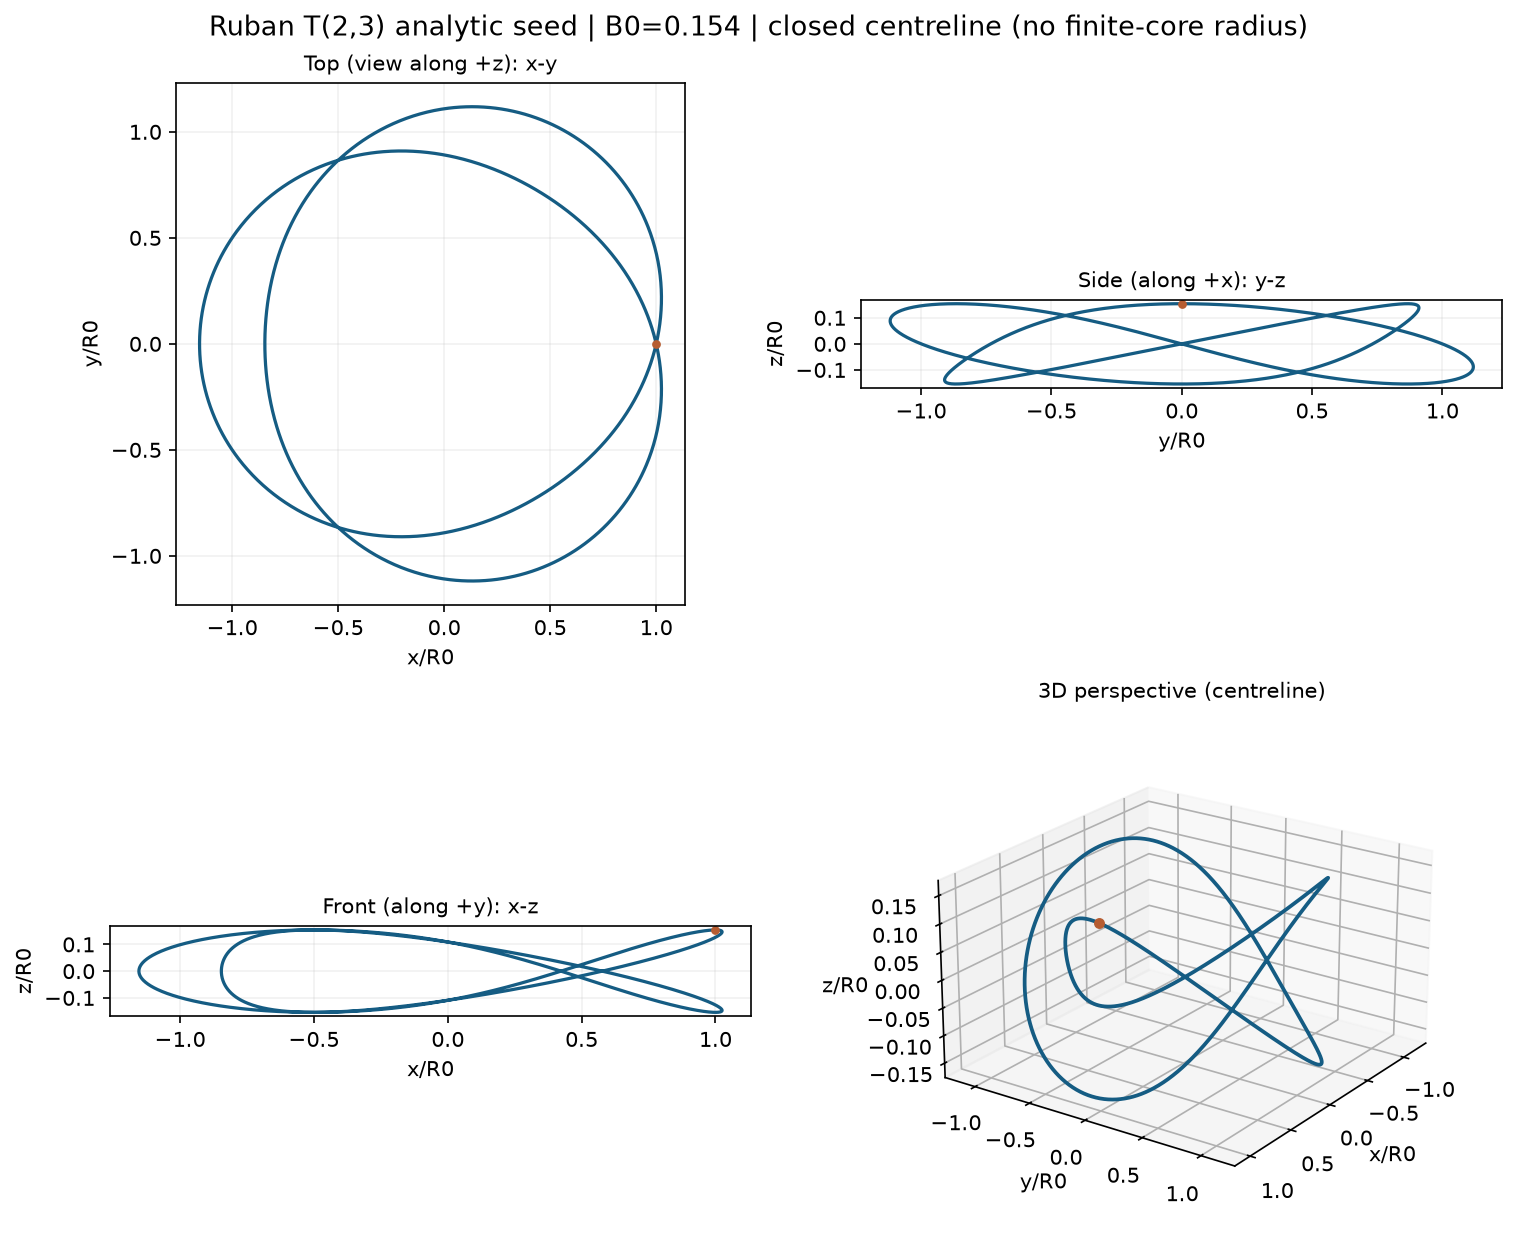
\includegraphics[width=.97\linewidth]{figures/seed_quad.png}
\caption{The analytical $T(2,3)$ seed, shown in the requested 2x2 array: top, side, front, and 3D perspective. The plotted line is the \emph{closed centerline only}; its line thickness is not a physical tube radius, and $\delta$ is a numerical regularization scale.}\end{figure}
\IfFileExists{figures/evolution.png}{\begin{figure}[H]\centering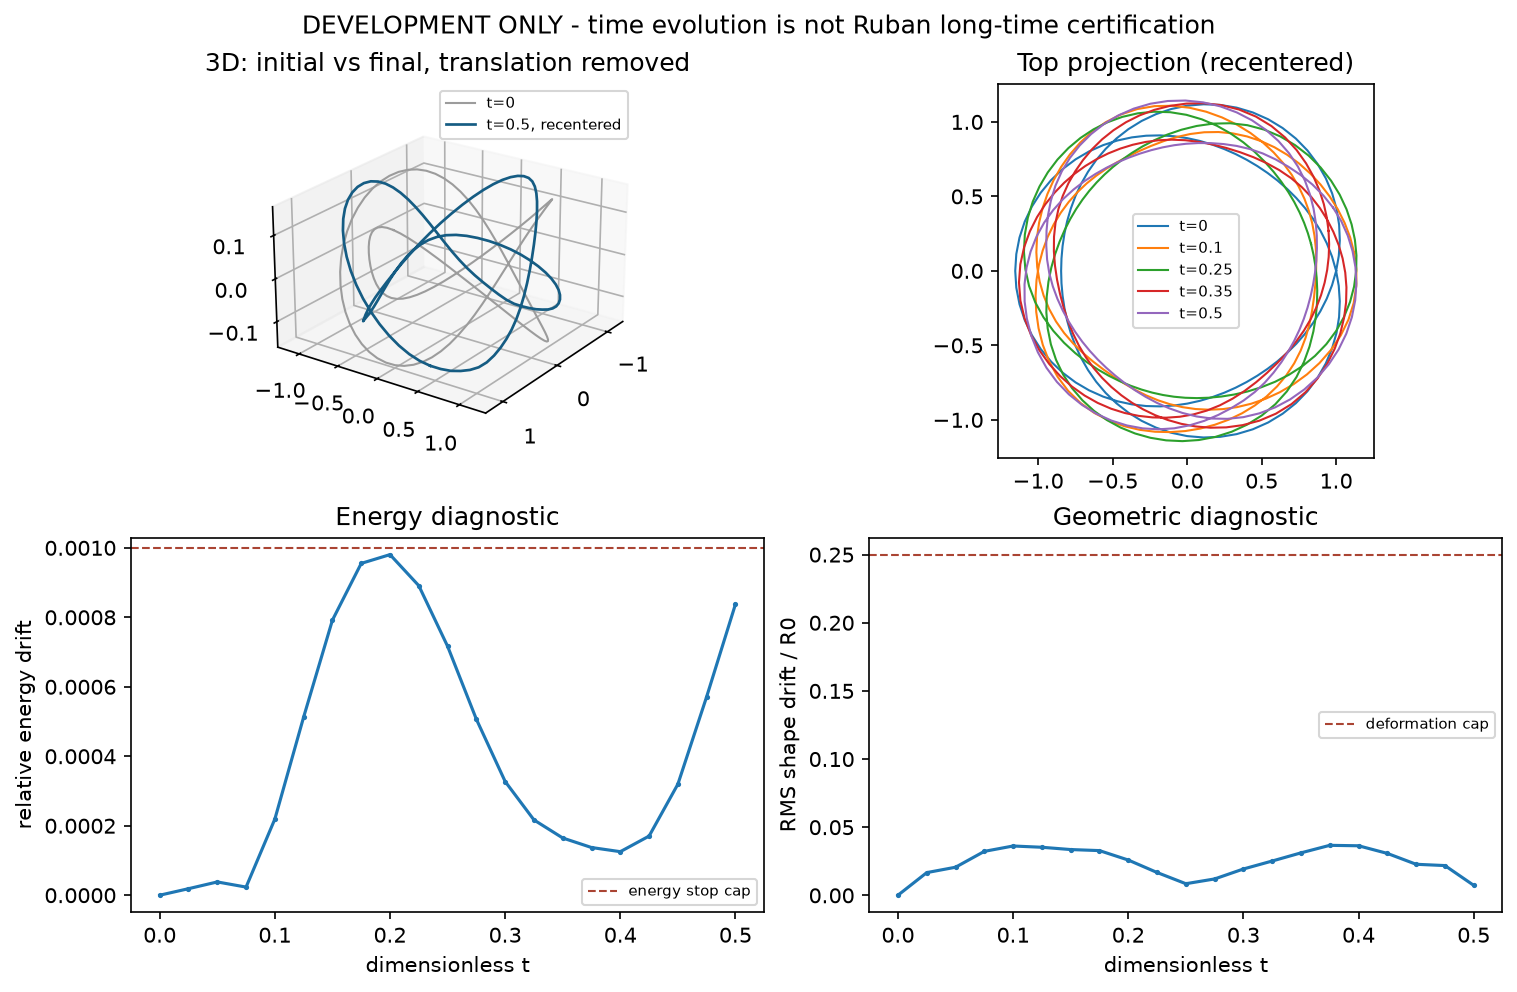
\includegraphics[width=.97\linewidth]{figures/evolution.png}\caption{Development-time evolution and diagnostics, referenced to the actual run. Short-time geometric persistence does not establish long-time stability.}\end{figure}}{}

% SST-REPORT-SECTION:INTERPRETATION

\section{Interpretation, limits, falsifiable predictions, and minimal follow-up experiments}
A short run that reaches its requested time with adequate energy conservation demonstrates only \emph{local numerical viability}. A long run that violates the energy gate is a numerical failure, not a physical refutation of the Ruban configuration. A positive long-time survival remains provisional until stable under space/time refinement. Minimum follow-up: canonical $B_0=0.154$ at equal $t=1$ for $N=128,256,512$, each with halved time steps; then verified $t=10$, $t=30$, and ultimately $t>300$. Internal twist and a dense background filament lattice are excluded from this version to isolate the published mechanism.
\subsection{Post-run discussion}
\IfFileExists{POST_RUN_DISCUSSION.tex}{\input{POST_RUN_DISCUSSION.tex}}{\emph{No post-run reinterpretation is silently inserted.}}

% SST-REPORT-SECTION:REPRODUCIBILITY

\section{Reproducibility and exact commands}
\begin{verbatim}
py -m pip install -r requirements.txt
run_all.cmd TEST
run_all.cmd SMOKE
run_all.cmd BASIC
run_all.cmd CONVERGE
run_all.cmd FULL
\end{verbatim}
\noindent \texttt{run\_all.cmd FREEZE}, \texttt{CERTIFY}, \texttt{REVEAL} are \textbf{refused} until an authenticated Framework v1.1.0 runtime instance has been installed and validated. Outputs are written to a version-specific directory and published in sibling ZIP/SHA-256 and PDF files. Existing output roots are not overwritten.

\section{References}
\begin{thebibliography}{99}
\bibitem{Ruban2018a} V.~P. Ruban (2018), ``Long-Lived Quantum Vortex Knots,'' \emph{JETP Letters} 107, 307--310, DOI: \url{https://doi.org/10.1134/S0021364018050120}.
\bibitem{Ruban2018b} V.~P. Ruban (2018), ``Quasi-Stable Configurations of Torus Vortex Knots and Links,'' \emph{Journal of Experimental and Theoretical Physics} 127, 581--586, DOI: \url{https://doi.org/10.1134/S106377611809008X}.
\bibitem{Saffman1992} P.~G. Saffman (1992), \emph{Vortex Dynamics}, Cambridge University Press, DOI: \url{https://doi.org/10.1017/CBO9780511624063}.
\bibitem{Gilbert2016} B. Gilbert (2016), \emph{Database of Ideal Knots 3--10 Crossings}, numerical dataset, entry 3:1:1, available from user-supplied library record.
\end{thebibliography}


\end{document}
